\documentclass[10pt,twocolumn]{article}
\usepackage[utf8]{inputenc}
\usepackage{graphicx}
\usepackage{amsfonts}
\usepackage[font=footnotesize, labelfont={sf,bf}, margin=0cm]{caption}
\usepackage{fancyhdr}
\usepackage{listings}
\pagestyle{fancy}
\lfoot{Analysing Mifare Classic}
\rfoot{Page \thepage}
\cfoot{Bastian Fredriksson}
\renewcommand{\headrulewidth}{0.4pt}
\renewcommand{\footrulewidth}{0.4pt}
\usepackage[dvipsnames]{xcolor}
\usepackage{hyperref}

\definecolor{codegreen}{rgb}{0,0.6,0}
\definecolor{codegray}{rgb}{0.5,0.5,0.5}
\definecolor{codepurple}{rgb}{0.58,0,0.82}
\definecolor{backcolour}{rgb}{0.95,0.95,0.92}
 
\lstdefinestyle{mystyle}{
    backgroundcolor=\color{backcolour},   
    commentstyle=\color{codegreen},
    keywordstyle=\color{magenta},
    numberstyle=\tiny\color{codegray},
    stringstyle=\color{codepurple},
    basicstyle=\footnotesize,
    breakatwhitespace=false,         
    breaklines=true,                 
    captionpos=b,                    
    keepspaces=true,                 
    numbers=left,                    
    numbersep=5pt,                  
    showspaces=false,                
    showstringspaces=false,
    showtabs=false,                  
    tabsize=2
}

\lstdefinestyle{tiny}{
    basicstyle=\ttfamily\tiny
}

\lstset{style=mystyle}

\newcommand\myshade{85}
\colorlet{mylinkcolor}{violet}
\colorlet{mycitecolor}{YellowOrange}
\colorlet{myurlcolor}{Aquamarine}

\hypersetup{
  linkcolor  = mylinkcolor!\myshade!black,
  citecolor  = mycitecolor!\myshade!black,
  urlcolor   = myurlcolor!\myshade!black,
  colorlinks = true,
}


\title{A case study in smartcard security\\Analysing Mifare Classic Rev. 1}
\author{
        \texttt{Bastian Fredriksson}\\
                \texttt{Faculty of IT, Monash University}\\
        \texttt{bfre12@student.monash.edu}\\
}
\date{May 16, 2016}

\begin{document}
\maketitle

\section{Glossary}
\textbf{Adversary} In cryptography, an adversary or attacker is a malicious opponent which tries to break the security of a system.\\
\textbf{Application Specific Integrated Circuit (ASIC)} is an integrated circuit constructed for a particular purpose.\\
\textbf{Bit} The smallest amount of information in a traditional computer. A bit can contain two different values, usually denoted by $0$ and $1$ respectively.\\
\textbf{Brute-force attack} An attack where an adversary tries to figure out a secret by enumerating all possible values.\\
\textbf{Byte} The smallest unit of addressable memory in a computer. A byte is a group of eight consecutive bits.\\
\textbf{CRYPTO-1} is the algorithm used by the Mifare Classic card for authentication and encryption.\\
\textbf{Field-programmable Gate Array (FPGA}) is an integrated circuit designed to be programmble by the customer after manufacture. An FPGA contains a large amount of logic gates and memory blocks, which makes it suitable for resource-intensive computations.\\
\textbf{International Standards Organisation (ISO)} is an organisation whose purpose is to create international standards for various products.\\
\textbf{Mifare Classic} (originally marketed as \textit{Mifare}, not to be confused with \textit{Mifare Classic EV1}) is a contactless smart card manufactured by NXP Semiconductors \cite{mifare-sheet}.\\
\textbf{Near Field Communication (NFC)} can be seen as an extension of RFID. NFC is mostly used by cellphones to communicate over short distances.\\
\textbf{Psuedo-Random Number Generator (PRNG)} is a cryptographic contruction for generating a seemingly random sequence of numbers.\\
\textbf{Radio Frequency Identification (RFID)} is a technology for wireless authentication where an \textit{RFID tag} (PCD) authenticates to an \textit{RFID reader} (PICC). The tag can for example be a smart card, cellphone or a car fob.\\
\textbf{Unique Identifier (UID)} is a non-unique 4-byte or unique 7-byte serial number used to differentiate between two Mifare cards \cite{mifare-sheet}.\\

\section{Introduction}
\textit{Mifare Classic MF1S50YYX}, or simply \textit{Mifare}, released by Philips (now NXP Semiconductors) in 1994 \cite{cid10}, is a contactless smart card used for cashless vending applications, access control to buildings, ticketing and payment systems. Most notably it is used as ticket and payment system in Taiwan (\textit{EasyCard} and in the Netherlands (\textit{OV-chipkaart}), and as public transport ticket system in many cities including London (\textit{Oyster Card}), Miami (\textit{Miami-Dade}), Perth (\textit{SmartCard}), Buenos Aires (\textit{SUBE}), Istanbul (\textit{Istanbul Kart}) and Stockholm (\textit{SL Access}).

\section{Card characteristics}
The Mifare Classic smart card is usually manufactured as a 53x85 mm plastic card containing a copper wire acting as antenna, attached to a small RFID chip as shown in figure \ref{fig:rfid-chip}.

\begin{figure}[ht]
\includegraphics[width=8cm]{rfid-chip.png}
\caption{An example of a typical RFID smart card made in plastic. The silhouettes of the copper wire and the chip can be seen by letting light shine through the card, for example by putting a torch behind it. The chip and the wire can be extracted from the card by melting the plastic with acetone.}
\label{fig:rfid-chip}
\end{figure}

The Mifare Classic is a passive RFID tag, meaning that it does not contain a battery. The RFID reader emitting an oscillating magnetic field which induces electricity into the copper wire powering up the chip. The maximum distance between tag and reader depends on the strength of the magnetic field, but is typically around 10 cm. Once the chip has powered up, it communicates on the 13.56 MHz frequency and offers a transaction speed up to 106 kB/s. A transaction between tag and reader takes approximately 100 ms \cite{mifare-sheet}.

The chip itself contains an ASIC microcontroller and a 1 kB or 4 kB flash memory which can be used to store data on the card. Mifare Classic with 1 kB and 4 kB memory is referred to as \textit{Mifare Classic 1K} and \textit{Mifare Classic 4K} respectively.

\section{Memory layout}
The memory is divided into sectors and blocks. Each sector is protected by two 48-bit keys, called \textit{key A} and \textit{key B}. The access control bits of each sector determines which key is required for each operation. Mifare Classic 1K is divided into 16 sectors with 64 bytes each. Every sector is divided into 4 blocks with 16 bytes each. The last block in each sector (called \textit{trailer}) contains the keys and the access control \textit{AC} bits. The first 6 bytes contains key A, the following 3 bytes contains the access control bits. The next byte (\textit{General Purpose Byte} or \textit{GPB}) is unused and can be used for storage. The last 6 bytes contains key B. The last 6 bytes can be used for storage if key B is not needed.

Mifare Classic 4K is divided into 40 sectors where the first 32 sectors are identical to the 4-block sectors found in Mifare Classic 1K. The remaining 18 sectors contains 16 blocks each, where each block is 16 bytes. The last block of each sector contains the keys and access control bits, following the same structure as for Mifare Classic 1K. 

The first block of the first sector (the \textit{manufacturer block}) contains the 4-byte or 7-byte UID of the card followed by a one byte checksum, given by the XOR of all bytes in the UID. The rest of the bytes in this block contains manufacturer specific data. The manufacturer block is usually read only \cite{an1304}. We refer to figure \ref{fig:mem1k} and \ref{fig:mem4k} for a detailed description of the memory layout.

\begin{figure}[ht]
\includegraphics[width=8cm]{mem1k.png}
\caption{Memory layout for a 4-block sector in Mifare Classic 1K and Mifare Classic 4K. The 1K memory contains a total of 16 sectors. Only sector 0 contains the manufacturer block (used for storage in the other sectors).}
\label{fig:mem1k}
\end{figure}

\begin{figure}[ht]
\includegraphics[width=8cm]{mem4k.png}
\caption{Memory layout for a 16-block sector in Mifare Classic 4K. The 4K memory contains a total of 32 sectors with 4 blocks each (identical to the sectors used in Mifare Classic 1K), and 18 sectors with 16 blocks each as shown above.}
\label{fig:mem4k}
\end{figure}

\subsection{Block types}
There are two types of blocks, data blocks and value blocks. Data blocks stores a 16 byte value in raw format. Value blocks stores a 4-byte signed integer in a fixed format which features error detection and correction. The value is stored in in little endian and negative values are written in two's complement. The value is stored three times for security \cite{mifare-sheet}. See figure \ref{fig:value-block} for details.

Value blocks are often used for storing sensitive information such as account balance. The purpose of storing the value three times is to prevent someone to tamper with the card by flipping individual bits using radiation.

\begin{figure}
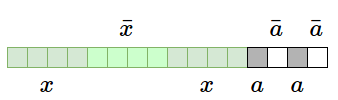
\includegraphics[width=8cm]{value-block.png}
\caption{Storage format for a value block. The block contains a 32-bit signed integer $x$. $\overline{x}$ denotes $x$ with all bits inverted. The last four bytes contains the 1-byte address $a$ of the block, repeated for times. This value is used for backup management \cite{mifare-sheet}.}
\label{fig:value-block}
\end{figure}

\subsection{Commands}
The microcontroller supports the commands \textit{read}, \textit{write}, \textit{increment}, \textit{decrement}, \textit{transfer}, and \textit{restore}. Read reads a single block from memory. If the sector trailer is read, the keys $A$ and $B$ (if present) will be masked out and replaced by zeroes. Write writes a single block to memory. The manufacturer block cannot be written to. Increment and decrement is used to increase or decrease the value of a value block by one. Transfer moves a block in memory into the internal register of the microcontroller. Restore moves the block stored in the internal register of the microcontroller to a block in memory.

\subsection{Access control}
The AC bits (3 bytes in total) defines read and write access to a sector based on the keys $A$ and $B$. One must be careful when setting the AC bits, since the microcontroller will lock the whole sector if an invalid format is detected. A triple of bits $(C1, C2, C3)$ defines access conditions for a single block (if the sector is a 4-block sector) or a chunk of four blocks (if the sector is a 16-block sector). The bits are stored both inverted and non-inverted for security purposes. For the format of the AC bits, see table 6 and figure 10 in the \href{http://www.nxp.com/documents/data_sheet/MF1S50YYX.pdf}{\textit{Mifare Classic 1K Data Sheet}} \cite{mifare-sheet} and \href{https://www.nxp.com/documents/data_sheet/MF1S70YYX.pdf}{\textit{Mifare Classic 4K Data Sheet}} \cite{mifare4k-sheet}. For access conditions to the sector trailer and the data blocks, see table 7 and table 8 in the data sheet.

\section{Linear Feedback Shift Register}
A \textit{Linear Feedback Shift Register (LFSR)} is a shift register used to generate a psuedo-random stream of bits. Due to its simplicity, it is commonly implemented directly in hardware, yielding a very fast PRNG. A PRNG based on a single LFSR is not cryptographically secure and should not be used in security critical applications. Given an $n$-bit LFSR it suffices to observe $2n$ consecutive bits from the output stream in order to deduce the generating polynomial \cite{weisstein1}. This polynomial, together with the last $n$ bits of the output stream can then be used to predict all subsequent bits.

A LFSR consists of an $n$-bit register. Each time a new bit of the output stream is produced (which normally happens once every clock cycle), a new \textit{input bit} is created by computing the exclusive or of the leftmost bit in the register with some fixed bits called \textit{taps}. The register is then shifted one step to the right. The leftmost empty position is filled with the input bit. The rightmost bit which was shifted out becomes the \textit{output bit}, the next bit in the output stream. The choice of taps corresponds to a polynomial in the ring $\mathbb{Z}_2[X]\setminus x^n$. For example, if the leftmost bit is bit $0$ and taps are bit $2$, $3$ and $5$, the generating polynomial becomes $p(x)=x^5+x^3+x^2+1$. The exponents indicates to the position of the tap and $x^0=1$ at the end represents the input bit (which is always a tap).

The choice of polynomial is important. One typically chooses an irreducible polynomial, which is guaranteed to generate all of the $2^n-1$ states before cycling back to its initial state. An irreducible polynomial is a polynomial which cannot be written as a product of two polynomials. Irreducible polynomials in a polynomial ring can be thought of as a prime number in a Galois field. Note that the state with all zeroes won't occur in the generated sequence, since this would lock up the LFSR.

Although a single LFSR is not cryptographically secure, it is possible to combine several LFSR to create a PRNG which can be used as a building block for cryptographic primitives such as stream ciphers. Several encryption algorithms uses an LFSR, including A5/1, A5/2, E0 and Trivium \cite{canniere}.

\section{Communication protocol}
\label{communication-protocol}
The communication protocol between tag (called \textit{PICC)} and reader (called \textit{PCD}) is loosely based on ISO/IEC-14443 Type A \cite{mifare-sheet} which describes the physical characteristics of the PICC and a protocol stack with three layers. Layer 1 regulates the signal power and signal interface and is responsible for the physical transmission of bits over the air \cite{iso14443-2}. Layer 2 describes an anticollision protocol where the PICC sends its UID to the PCD, whereby the PCD selects the card. This makes it possible for more than one card to operate in the field at the same time \cite{iso14443-3}. Layer 3 describes the transmission protocol between PIC and PCD once a connection has been established \cite{iso14443-4}.

\section{CRYPTO-1}
CRYPTO-1 is a symmetric stream cipher used by the Mifare Classic card for encryption and authentication. The cipher uses a 48-bit pre-shared key for encryption and decryption. Hardware-analysis shows that the cipher is very small, about $8.5$ times smaller than the most compact AES-implementation. The cipher is also very fast, producing one bit of keystream each clock cycle. However, cryptoanalysis shows that the design of the cipher contains serious weaknesses \cite{nohl08}. A GPLv2 implementation written in C called CRAPTO-1 was released in 2008.

\subsection{Keystream generation}
At the heart of the cipher is the keystream generator depicted in figure \ref{fig:crapto-prng}. The keystream generator is made up of a 48-bit LFSR holding the cipher state, and six non-linear functions $(f_1, f_2\ldots f_6)$. At each clock cycle, the first four odd bits, starting at bit 9, is fed into $f_1$ - the next four odd bits are fed into $f_2$ and so on. The last four odd bits are fed into $f_5$. The output of $f_1, f_2\ldots f_5$ is fed into $f_6$ which outputs one keystream bit. Next, the taps of the LFSR are combined using exclusive or to produce a new input bit $b$ and the LFSR shifts one step to the left. The leftmost output bit is discarded and the empty rightmost bit is filled with $b$. We refer to \cite{tan09} section 4.1.1 for formulas to the filter functions $f_1, f_2\ldots f_6$ and the generating polynomial for the LFSR.

\begin{figure}
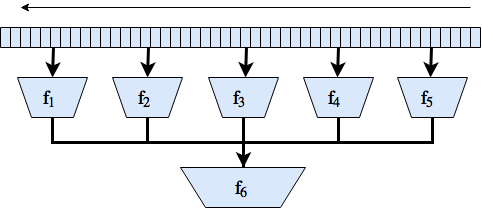
\includegraphics[width=8cm]{crapto1.png}
\caption{Overview of the PRNG in the Crypto1 stream cipher. The PRNG consists of a 48-bit LFSR and six non-linear filter functions.}
\label{fig:crapto-prng}
\end{figure}

\subsection{Psuedo-random number generator}
The Mifare Classic Psuedo-random number generator is a separate circuit which is responsible for creating nonces used in the challenge-response protocol which authenticates tag and reader. The PRNG can be seen as a 32-bit register $(b_1, b2, \ldots b_{31})$ which contains a 16-bit LFSR. The snapshot of the register at time $i$ gives nonce number $i$ in the psuedo-random sequence. The next number in the sequence is given by a successor function $suc(x)$. This function is implemented in the Crapto1 library as \verb!prng_successor!.

Every 9.44 $\mu$s the PRNG computes the next state of the register by computing the exclusive or of the four taps $b_{16}, b_{18}, b_{19}, b_{21}$ to form the next input bit $b_\oplus$. The register is then shifted one step to the left and the new input bit is inserted to the right. Note that the function \verb!prng_successor! returns the register with each byte shifted one bit to the right. More formally, if the input state $x$ is $x_1, x_2, x_{31}$, the return value from the function call \verb!prng_successor(x, 1)! becomes $x_8, x_1\ldots x_7$, $x_{16}, x_9\ldots x_{15}$, $x_{24}, x_{17}\ldots x_{23}$, $x_\oplus, x_{25}\ldots x_{31}$. See figure \ref{fig:prng-design} for more details.

\subsection{Challenge-response protocol}
\label{challenge-response}
We are now ready to describe the challenge-response protocol, in which the tag and reader proves knowledge of the secret key. After the anti-collision phase 
completes, the reader sends a command which tells the card which sector it wants to authenticate to and which key it wants to use. The tag responds with a 32-bit tag nonce $N_T$ generated using the PRNG. The reader answers with its own challenge $N_R$ and a response $A_T = suc^{64}(N_T)$ (the 64th successor of $N_T$), both encrypted under the secret key. Note that the reader challenge $N_R$ is supposed to be random in the real protocol, but this value can be chosen freely by the attacker. 

The tag checks that the reader knows the secret key by computing $Dec(A_T) = suc^{64}(N_T)$. If the authentication succeeded, the tag proceeds by answering with $A_T = suc^{96}(N_T)$ encrypted using the secret key. If the authentication failed ($Dec(A_T) \neq suc^{64}(N_T)$), the card remains silent.

After the reader receives $A_T$ it checks whether $Dec(A_T) = suc^{96}(N_T)$. This completes the challenge-response protocol, and both tag and reader can now communicate with each other. Note that $N_R$ is not used directly in this protocol, this value is shifted into the cipher state and will affect what the keystream looks like.

\subsection{Cipher initialisation}
The tag and reader must reach the same cipher state after the challenge-response protocol has completed in order to be able to properly encrypt and decrypt the communication that follows. The parameters used for cipher initialisation is the 48-bit secret sector key $K$, the tag nonce $N_T$, the reader nonce $N_R$ and the UID $u$ of the tag. 

The LFSR of the cipher is first initialised using $K$ with the most significant bit the leftmost position. $N_T = (N_{T_0}, N_{T_1} \ldots N_{T_{31}})$ and $u = (u_0, u_1 \ldots u_{31})$ is then shifted into the register together with the next feedback bit $b_i$. This means, $b \oplus N_{T_i} \oplus u_i$ is inserted into the rightmost position $\forall i \in [0, 31]$. Then $N_R = (N_{R_0}, N_{R_1} \ldots N_{R_31})$ is shifted in together with the feedback bit. Since the reader knows $u$ which is sent by the tag in the anticollision phase, the secret $K$ and $N_T$ (which is sent unencrypted from the tag), the reader will be able to initialise the cipher after recieving $N_T$ from the tag, and produce the keystream required to encrypt $N_R$ and $A_R$. Since the tag knows its id $u$ and the secret $K$, it will be able to produce 32 bits of keystream, enough to decrypt the nonce $N_R$ sent by the reader. This value can then be used to decrypt $A_R$ and finalise the initialisation of the cipher. 

\section{Weaknesses}
\label{flaws}
Reverse engineering of the chip and cryptanalysis of the cipher has discovered several flaws which will be discussed below. Some of the flaws are due to the design of the psuedo-random generator, others has to to with the protocol or weaknesses with the cipher itself. 
\begin{enumerate}
    \item \textbf{Short key length}\\
    \textit{Problem} Since the key is only 48-bits, it will be possible to brute-force the key in about one week on a standard PC. As long as the design of the cipher remained secret, brute-force attacks were not possible due to the slow hardware in Mifare Classic. However, once the algorithm was reverse engineered, it became possible to implement the cipher in software and run it on any hardware which speeds up the attack. The cipher is designed to be very small, and can be implemented very efficiently on an FPGA \cite{nohl08_yt}. Brute-force attacks on Mifare Classic is discussed in more detail in section \ref{brute-force}.\\
    \textit{Mitigation} The designers of Mifare Classic should have used a longer key (arguably, the key size might have been a security vs cost tradeoff since the key length affects many other aspects of the chip, however a 48-bit key is unfortunately too short to provide any security against an adversary). A proper keysize would be at least 85 bits to be resilient against brute-force attacks.
    \item \textbf{Short PRNG cycle}\\
    \textit{Problem} Although the PRNG spits out a 32-bit number, since the construction is based upon a 16-bit LFSR, the efficient amount of entropy is only 16 bits, not 32 bits. Consequently, the psuedorandom sequence generated by the PRNG does only consist of $2^{16}=65536$ numbers. Since the PRNG switches state every 9.44 $\mu$s, the psuedo-random sequence repeats itself after $\approx619$ ms.\\
    \textit{Mitigation} More taps should be chosen for the generating polynomial, thus if chosen wisely (such that the corresponding generating polynomial is irreducible) the length of the psuedorandom sequence would be much longer and repeat itself after about 11 hours. This could be implemented with modest changes to the chip, and neither the cipher nor the protocol would have to be changed.
    \item \textbf{$N_T$ is easily reproduced}\\
    \textit{Problem} Since the attacker controls time, and the psuedo-random number generated by the PRNG only depends on the time elapsed between the tag being powered up and the time the tag was challenged, the attacker can efficiently reproduce the same random number over and over again \cite{nohl08_yt}. The fact that the PRNG resets its internal state on startup makes this attack easier.\\
    \textit{Mitigation} The designers of the PRNG could have designed the chip such that it does not reset its internal state on startup. This would make the psuedorandom sequence much harder to predict, and no changes to the protocol or cipher itself would be required.
    \item \textbf{Leftmost bit of the cipher is not a tap}\\
    \textit{Problem} The leftmost bit $x_0$ of the cipher is not used to generate the feedback bit. This makes it possible to create a rollback function (see \cite{garcia09}) which, given the internal state of the cipher at any point in time, rolls back the internal state by one step. By repeating this rollback function several times, one will eventually arrive at the initial state of the cipher which contains the secret sector key $K$.\\
    \textit{Mitigation} The bit $x_0$ should have been used as a tap in the generating polynomial.
    \item \textbf{Parity bits leaks information}\\
    \textit{Problem} The ISO-14443-A standard discussed in section \ref{communication-protocol} mandates that each byte should be accompanied by a parity bit. The parity bit is an error detecting code which should be 1 if the hamming weight of the byte is odd, and 0 otherwise. That means, each 32 bit word will be sent together with four parity bits, one for each byte. When the tag receives $N_R$ and $A_R$ encrypted by the reader, the tag will check the correctness of the parity bits before validating the response $A_R$. If the parity bits are correct, but the response is invalid, the tag will send \verb!NACK! (0x5) back to the reader in encrypted form. By XORing the encrypted message with the known plaintext, four keystream bits can be retrieved.\\
    \textit{Mitigation} The tag should send \verb!NACK! unencrypted or not answer at all.
    \item \textbf{Statistical weaknesses in the cipher}\\
    \textit{Problem} The cipher contains statistical weaknesses. This was exploited by Nicolas Curtois in his Dark Side Attack discussed in \cite{curtois09}.\\
    \textit{Mitigation} This problem is due to the poor construction of the non-linear functions $f_1, f_2\ldots f_6$ used to mix state of the LFSR. Unfortunately, this is a major flaw with the cipher itself and not easily fixed.
    \item \textbf{Nested authentications}\\
    \textit{Problem} If the reader already has authenticated to one sector, and tries to authenticate to another, the tag will repeat the challenge-response protocol as discussed in \ref{challenge-response}. However, this time, the tag nonce is sent encrypted. Due to the short PRNG cycle, there are only $2^{16}$ different nonces. Combined with the parity bit information leak, the number of possible nonces can be reduced to $2^{13}$ \cite{garcia09}. Once the reader guesses the correct nonce, 32 bits of keystream can be recovered. This information can then be used to deduce the secret key for the new sector. This attack is called the nested-authentication attack and will be discussed in section \ref{attack-tools}.\\
    \textit{Mitigation} This problem can be mitigated by always sending the tag nonce unencrypted. However, the attack is made possible by a combination of flaws, both with the PRNG and the cipher itself.
\end{enumerate}

Apart from the above mentioned problems, there are some other minor design issues with the Mifare Classic chip. Since the chips themselves cannot be reprogrammed, the smartcards themselves should be replaced by a newer version which is more secure. Any data on the card should be considered compromised. Any sensitive data stored on the card should be stored encrypted, so it cannot be tampered with by an attacker. In practice many systems, such as \textit{SL Access public transport} in Stockholm, employs a central database which contains a copy of the contents of the card. Readers which are offline, for example readers installed on buses, are synced regularly with the central database. Every time the customer taps his tag onto the reader, the information stored on the card is crosschecked with the information stored in the database. This makes it practically impossible to cheat if the system is deployed correctly. However, since the same keys are typically used on all cards, it is possible for an attacker to wirelessly pickpocket or clone cards from other customers (using for example Curtois dark-side attack which does not require interaction with a reader \cite{curtois09}). The SL Acccess-system mitigates this type of attack by looking for "impossible travels". If the same card UID is detected by a reader on two different stations, and the time between the taps is in some sense short, the UID will be blacklisted by the system. This makes it difficult to travel with a card shared by different users, and almost impossible to travel using a stolen card, in particular if the owner of the card travels often.

Customers can also protect someone from stealing the contents of their card by putting the in a wallet with electromagnetic shielding. Many wallets has uses a foil of metal to achieve this. 

\section{Brute-force attack}
\label{brute-force}
In this section we will briefly discuss how to exploit the flaws found in section \ref{flaws}. Due to the short key length, the most obvious attack is a brute-force attack where the attacker tries to guess the correct sector key. The attacker powers up the tag and receives its "random" challenge $N_T$, whereby the attacker answers with eight random bytes for $Enc(N_T)$ and $Enc(A_R)$ and eight random parity bits, one for each byte. For each byte, the probability for the parity bit being correct is exactly $\frac{1}{2}$. That means, the probability for all parity bits being correct and the tag responding with \verb!NACK! will be $\frac{1}{2^8}=\frac{1}{128}$. The attacker can uniquely determine a key after six successful authentication attempts. This means that the attacker only needs to do on average $256*6=1536$ authentication attempts which takes roughly one second \cite{garcia09}.

The offline attack consists of enumeration of all possible $2^{48}-1$ keys. Assuming that the attacker has recorded each successful authentication attempt in a table $T$; For each key, the attacker shifts in the card UID and $N_T$ into the Crypto1 register and computes a 32-bit keystream which can be used to decrypt the reader nonce $N_R$. If the parity bits are valid, the attacker proceeds by shifting $N_R$ into the register and decrypting $A_R$. If the parity bits of $A_R$ are correct and the response is valid ($suc^{64}(N_T)=A_R$), the attacker proceeds with these checks using the next authentication attempt. The correct key has been found the key produces the correct parity bits and the correct response for each of the six authentication attempts. 

Although an attacker must traverse each of the $2^{48}-1$ different keys, the speed of the attack can be increased by distributing the computation between many machines. For a description of the attack in psuedocode, see the appendix.

\begin{figure}[ht!]
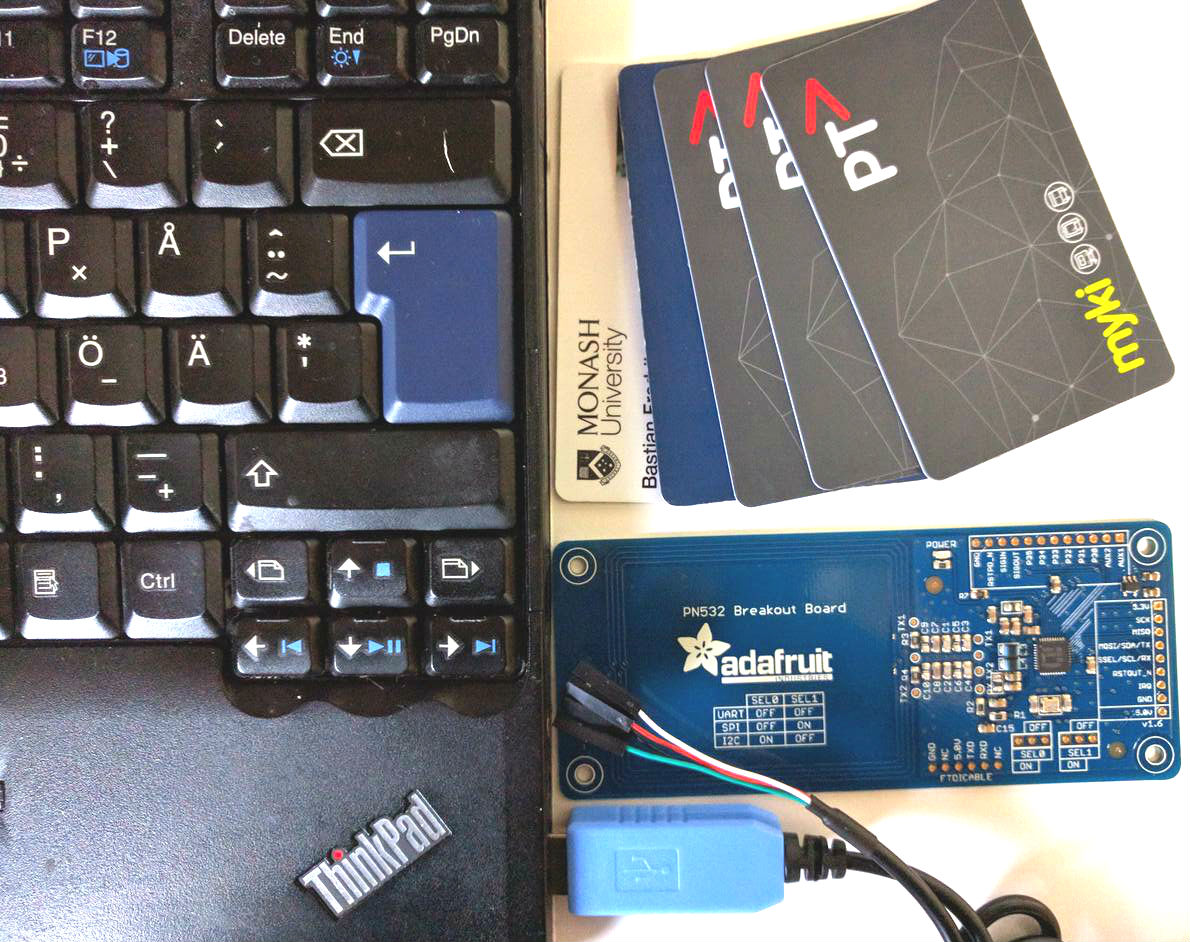
\includegraphics[width=8cm]{nfc-tools.jpg}
\caption{Equipment for reading and writing RFID tags. In this case an Adafruit PN532 breakout board connected via USB to a ThinkPad X201.}
\label{fig:nfctools}
\end{figure}

\section{Hacking techniques}
\label{attack-tools}
In this section we will discuss various tools and techniques for hacking Mifare Classic. The most efficient attacks are \textit{the nested-authentication attack} \cite{garcia09} and \textit{Curtois dark-side attack} \cite{curtois09}. The nested-authentication attack is faster than Curtois dark-side attack but requires knowledge of at least one sector key. There are software implementations available for both attacks, built on top of the NFC communication library \verb!libnfc! and the Crypto1 implementation \verb!Crapto1!.

To hardware required to perform the attack is a laptop or desktop computer (typically running some distribution of Linux), an RFID reader such as Proxmark 3, Touchatag ACR122 or Adafruit PN532 breakout board connected via USB or hooked up to a Raspberry Pi. It is recommended not to run the attack inside a virtual machine since this the attack relies heavily on precise timing to generate make the tag generate the correct tag nonce $N_T$.

If the goal is to make a complete clone of the card, one also needs an RFID card with a writable sector 0. Such cards can be bought from online retailers such as eBay or AliExpress. Another useful tool for reading tags is an NFC powered cellphone such as LG Nexus 5X with \textit{Mifare Classic Tool} installed. This app makes it easy to dump the contents of the card on the fly and get access conditions in a human-readable format based on the access bits of a sector. However these operations requires knowledge of the keys to the card, as far we can tell, since Android does not support \verb!libnfc! out of the box, separate hardware is required to break the keys.

In a typical attack scenario, the attacker wants to clone or change the contents of a card containing some sensitive data such as a public transport ticket or credits. Assuming that the attacker does not know anything about the sector keys used and only has access to the card itself (that is, the attacker is not able to sniff the communication between tag and reader), they would proceed as follows:
\begin{enumerate}
    \item First determine if the any of the sectors uses one of the default factory keys. Mifare Classic Tool with the \verb!extended-std.keys! list will do the trick.
    \item If at least one key was recovered, use the nested-authentication attack to recover the rest of the keys. If not, use Curtois dark-side attack to recover one sector key and then proceed with the nested-authentication attack.
    \item Once the keys are recovered, the attacker has unlimited R/W access to the card and can dump the contents of the card to disk, flip individual bits or clear whole sectors.
\end{enumerate}

Curtois dark-side attack is implemented in the library \verb!MFCUK! (Mifare Classic Universal Toolkit) and the nested-authentication attack is implemented in the library \verb!MFOC! (Mifare Classic Offline Cracker) \cite{gupta}. Before we begin, one should install \verb!libnfc!. If you use for example Ubuntu, this library will be available in the repository as \verb!libnfc-dev!, but we recommend that you compile the library from scratch since the pre-compiled package usually lacks the drivers needed.

\lstinputlisting[language=bash]{hack1.txt}

Once \verb!linfc! is installed, connect your RFID reader and check that the connection is working by issuing the command \verb!nfc-list!. Once you have assured that the connection is working properly, proceed by compiling \verb!MFCUK! and \verb!MFOC!.

\lstinputlisting[language=bash]{hack2.txt}

Typical use of \verb!mfcuk! would look something like \verb!mfcuk -C -R 0:A -v 2!. This will recover key A from sector 0, the \verb!-v! flag enables verbose mode to know what the tool is doing during the attack. Once a key has been recovered, one can continue to dump the rest of the keys to file with \verb!mfoc -O keys.mfd!. 

\section{Conclusion}
The internal machinery of Mifare Classic remained a trade secret for over ten years, until Nohl et al. \cite{nohl08} reverse engineered the chip in 2007. Once the algorithm and psuedo-random number generator became public, cryptographers quickly discovered ways to recover the secret key. Many different attacks were published, starting with offline attacks which required precomputation of large tables, ending with a total break where the attacker essentially could recover the secret key in less than a second using his cellphone. 

Mifare Classic is quite well covered at this point, and it is unlikely that any new attacks will be discovered. It is possible that existing attacks will be refined, but it is not probable since the technology is considered a legacy product. Mifare Classic is still in use, but tends to be in disfavour when new systems are deployed. Hence, researchers have started to look at the newer products made by NXP, such as Mifare Plus, Mifare DESFire and Mifare Ultralight. Any attacks for Mifare Classic cannot be extended to these cards, since NXP has switched to other cryptographic algorithms. For example, Mifare Plus uses AES with a 128 bit key and Mifare DESFire and Mifare Ultralight uses Triple-DES. These card implementations appears to be more robust than Mifare Classic, but time will tell for how long.

\bibliographystyle{acm}
\bibliography{references}

%%%%%%%%%%%%%%%%%%%%%%%%%%%%%%%%%%%%%%%%%%%%%%%%%%%%%%%%%%%%%%%%%%%%%%%%%%%%
\onecolumn
\section{Appendix}
\lstinputlisting[language=C]{prng_test.c}
\newpage
\begin{figure*}[ht] % lack of star here wasted 10 minutes LOL
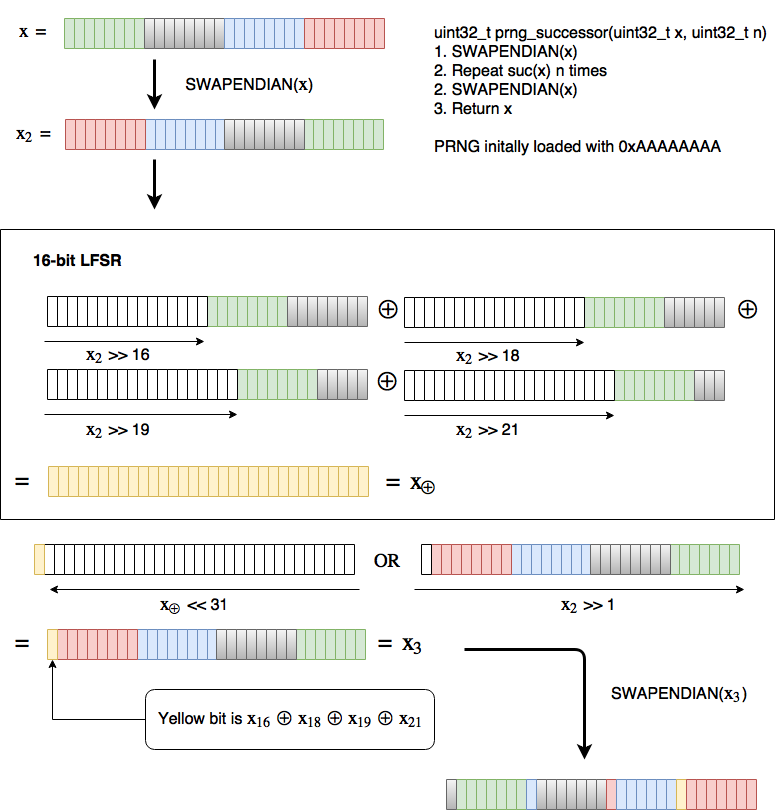
\includegraphics[width=16cm]{prng-design.png}
\caption{Design of the psuedo-random number generator in Mifare Classic. The PRNG is based on a 16-bit LFSR with the tap bits $x_{16}$, $x_{18}$, $x_{19}$, and $x_{21}$.}
\label{fig:prng-design}
\end{figure*}
\newpage
\lstinputlisting[language=Python]{brute-force.c}
Psuedocode describing a brute-force attack against the tag. This attack requires 1536 authentication attempts and a large offline computation.
\newpage
\lstset{style=tiny}
\lstinputlisting[language=C]{crapto-prng-test.txt}
The first 80 states of the Mifare Classic psuedo-random number generator starting at \verb!0xff00ff!. One can clearly see how the next state is created by shifting the previous state to the left.
\end{document}
